\clearpage{\pagestyle{empty}\cleardoublepage}

\chapter{\wbx\ analysis: SR cut-flow}\label{app:wbxSR}

In this appendix some more information about the cut-flow in the
signal regions for the \wbx\ analysis is given. We remind in 
Table~\ref{tab:wbxselectionBIS} the signal regions definition.
In the following sections the selected number of events selected in the
electron (Table~\ref{tab:cftabELE}) and muon (Table~\ref{tab:cftabMUON})
channels are reported, and the distribution of the discriminant variable
\mreco\ is shown in the various signal regions.

\begin{table}[h!]
\begin{center}
\begin{tabular}{lll}
\toprule
Selection & Signal Region & Requirements \\
\midrule
Preselection & & One electron or muon  \\
             & & $\met >20\gev$, $\met +m_{\rm T}>60\gev$ \\
             & & $\geq 4$ jets, $\geq 1$ $b$-tagged jets \\
\midrule
\loose\ selection & SR0 & Preselection  \\
                  & SR1 & +\hskip5ex$\geq 1~W_{\rm had}$ candidates \\
                  & SR2 & +\hskip5ex$\HT>800\gev$ \\
                  & SR3 & +\hskip5ex $\pt(b_1) > 160\gev$\\
                  & SR4 & +\hskip5ex$\pt(b_2) >80\gev$ \\
                  & SR5 ($\equiv$\loose) & +\hskip5ex$\Delta R(\ell,\nu)<1.2$ \\
\midrule
\tight\  selection & SR5 & \loose\ selection \\
     	      & SR6 &  +\hskip5ex min$\Delta R(\ell,b)>1.4$\\
              & SR7 ($\equiv$\tight) & +\hskip5ex min$\Delta R(W_{\rm had},b)>1.4$ \\
\bottomrule
\end{tabular}
\caption{Summary of event selection requirements.}
\label{tab:wbxselectionBIS}
\end{center}
\end{table}

\newpage

\section{Event yields in the electron and muon channels}\label{app:wbxSR_yields}


\begin{table}[h!tb]\centering
\resizebox{1.\textwidth}{!}{
        \begin{tabular}{l c c c c } \toprule\toprule
 & $T\bar{T}$ (600) chiral 		 & $t\bar{t}$ MC@NLO 		 & non-$t\bar{t}$ 		 & Data 		 \\ \midrule 
  Preselection  & $189.67 \pm 4.83$  & $92135.41 \pm 189.70$  & $29216.10 \pm 228.75$  & $117565.00 \pm 342.88$ \\ 
 +$\geq 1~W$ candidate  & $88.83 \pm 3.28$  & $2918.44 \pm 33.94$  & $677.93 \pm 31.70$  & $3845.00 \pm 62.01$ \\ 
 +$\HT>800\gev$  & $86.26 \pm 3.25$  & $726.61 \pm 17.78$  & $274.47 \pm 22.04$  & $1109.00 \pm 33.30$ \\ 
 +$\pt(b_1) > 160\gev$  & $74.79 \pm 3.01$  & $355.86 \pm 12.38$  & $153.24 \pm 15.91$  & $560.00 \pm 23.66$ \\ 
 +$\pt(b_2) >80\gev$  & $58.54 \pm 2.68$  & $195.30 \pm 9.08$  & $62.49 \pm 10.83$  & $263.00 \pm 16.22$ \\ 
 +$\Delta R(\ell,\nu)<1.2$  & $49.24 \pm 2.47$  & $119.27 \pm 6.93$  & $25.03 \pm 5.71$  & $164.00 \pm 12.81$ \\ 
 +min$\Delta R(\ell,b)>1.4$  & $38.02 \pm 2.16$  & $10.94 \pm 2.30$  & $11.01 \pm 2.18$  & $27.00 \pm 5.20$ \\ 
 +min$\Delta R(W,b)>1.4$  & $30.49 \pm 1.94$  & $4.34 \pm 1.63$  & $4.25 \pm 1.69$  & $18.00 \pm 4.24$ \\ 
\bottomrule\end{tabular}}
        \caption{
Number of observed events, integrated 
          over the whole mass spectrum, compared to the Standard Model expectation for
          the electron channel
          in the Signal Regions (see Table~\ref{tab:wbxselectionBIS} for the
        region definitions).
          The expected signal yields for a chiral 
          fourth-generation $\T$ quark with $m_{\T}=600\gev$ are also shown.
          The quoted uncertainties are only statistical.}\label{tab:cftabELE}
\end{table}


\begin{table}[h!tb]\centering
\resizebox{1.\textwidth}{!}{
        \begin{tabular}{l c c c c } \toprule\toprule
 & $T\bar{T}$ (600) chiral 		 & $t\bar{t}$ MC@NLO 		 & non-$t\bar{t}$ 		 & Data 		 \\ \midrule 
  Preselection  & $189.96 \pm 4.94$  & $109557.56 \pm 209.09$  & $36746.64 \pm 273.68$  & $144316.00 \pm 379.89$ \\ 
 +$\geq 1~W$ candidate  & $79.46 \pm 3.14$  & $3417.09 \pm 37.47$  & $756.58 \pm 33.26$  & $4556.00 \pm 67.50$ \\ 
 +$\HT>800\gev$  & $74.98 \pm 3.06$  & $848.26 \pm 19.52$  & $279.84 \pm 20.54$  & $1250.00 \pm 35.35$ \\ 
 +$\pt(b_1) > 160\gev$  & $63.55 \pm 2.82$  & $456.26 \pm 14.10$  & $138.84 \pm 12.77$  & $663.00 \pm 25.75$ \\ 
 +$\pt(b_2) >80\gev$  & $47.91 \pm 2.45$  & $241.55 \pm 10.19$  & $55.94 \pm 8.65$  & $335.00 \pm 18.30$ \\ 
 +$\Delta R(\ell,\nu)<1.2$  & $38.74 \pm 2.21$  & $144.45 \pm 7.73$  & $24.64 \pm 4.30$  & $184.00 \pm 13.56$ \\ 
 +min$\Delta R(\ell,b)>1.4$  & $29.08 \pm 1.93$  & $15.73 \pm 2.78$  & $10.54 \pm 3.01$  & $34.00 \pm 5.83$ \\ 
 +min$\Delta R(W,b)>1.4$  & $23.43 \pm 1.73$  & $5.69 \pm 1.89$  & $5.95 \pm 2.56$  & $19.00 \pm 4.36$ \\ 
\bottomrule\end{tabular}}
        \caption{Number of observed events, integrated 
          over the whole mass spectrum, compared to the Standard Model expectation for
          the muon channel 
          in the Signal Regions (see Table~\ref{tab:wbxselectionBIS} for the
        region definitions).
          The expected signal yields for a chiral 
          fourth-generation $\T$ quark with $m_{\T}=600\gev$ are also shown.
          The quoted uncertainties are only statistical.}\label{tab:cftabMUON}
\end{table}


\section{Reconstructed mass in the SRs}\label{app:wbxSR_mreco}

Figure~\ref{fig:mrecoSRs} shows the progress of signal selection
and background rejection in the various signal regions that progressively
approach the final \tight\ selection.

\begin{landscape}
\begin{figure}[htb]\begin{center}
\vskip-1cm
	\subfigure[]{\label{fig:mrecoSR1}
  	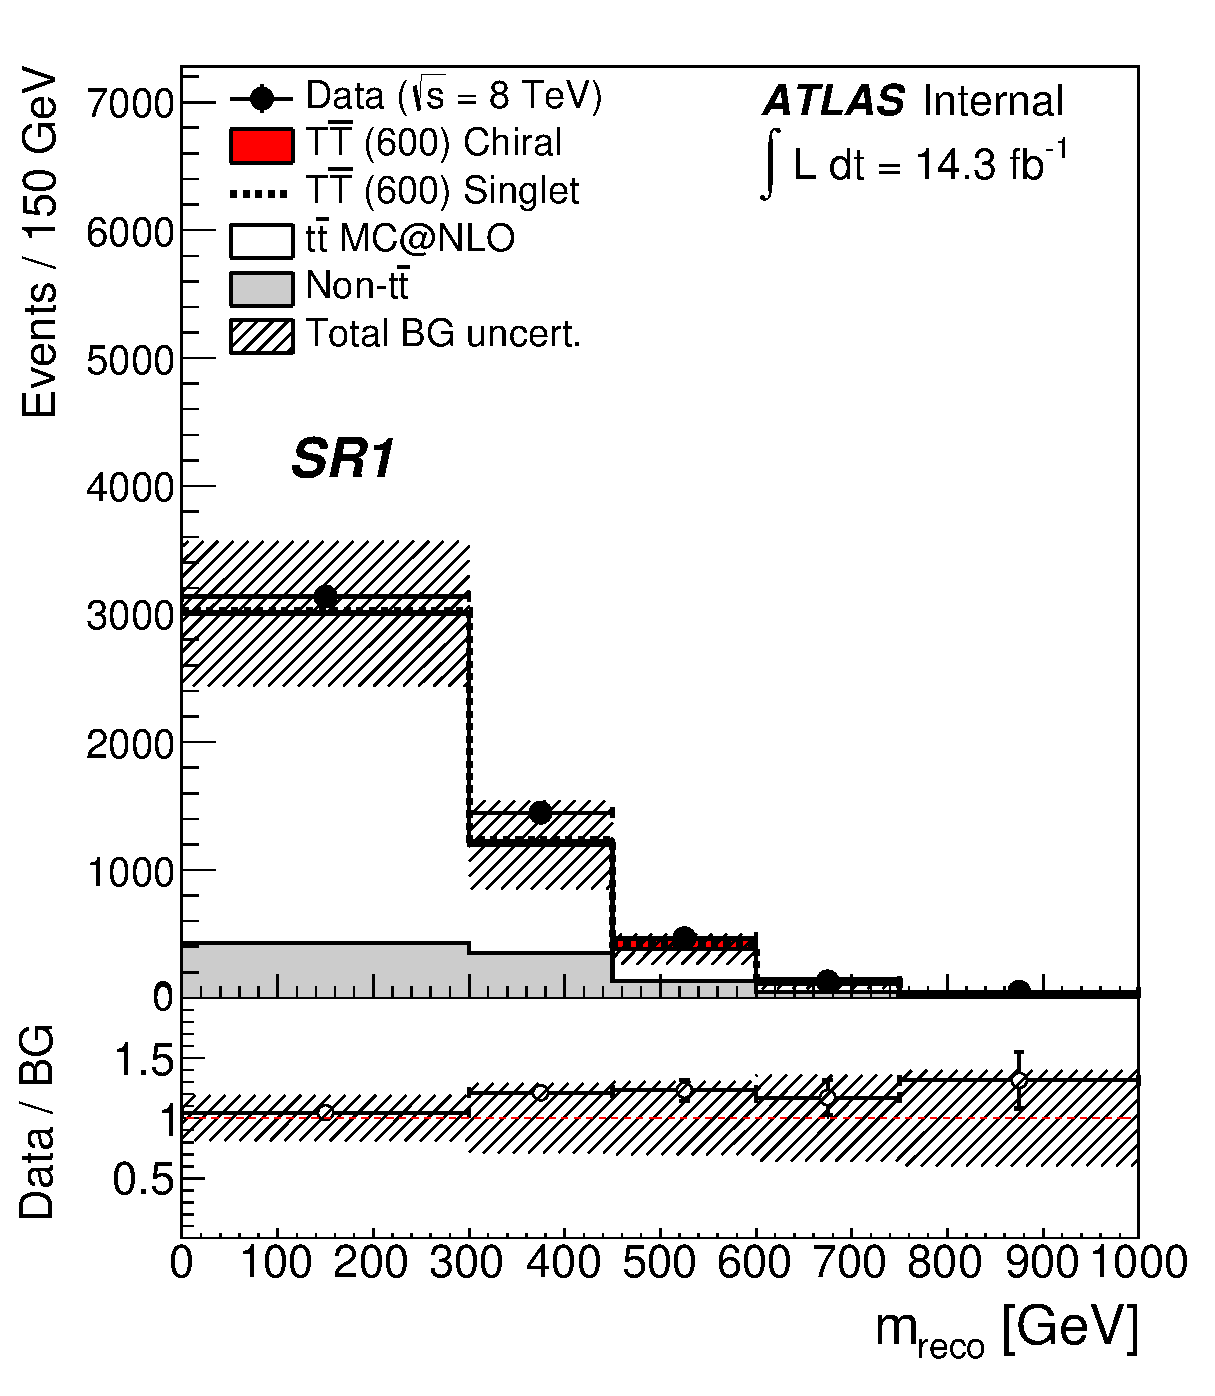
\includegraphics[width=0.37\textwidth]{wbx_analysis_14ifb/figures/THESIS_c6_cutflow/VLQAna_WbX_1W_MWb_4_ELEMUON_cutflow1_NOMINAL.eps}}
	\subfigure[]{\label{fig:mrecoSR2}
  	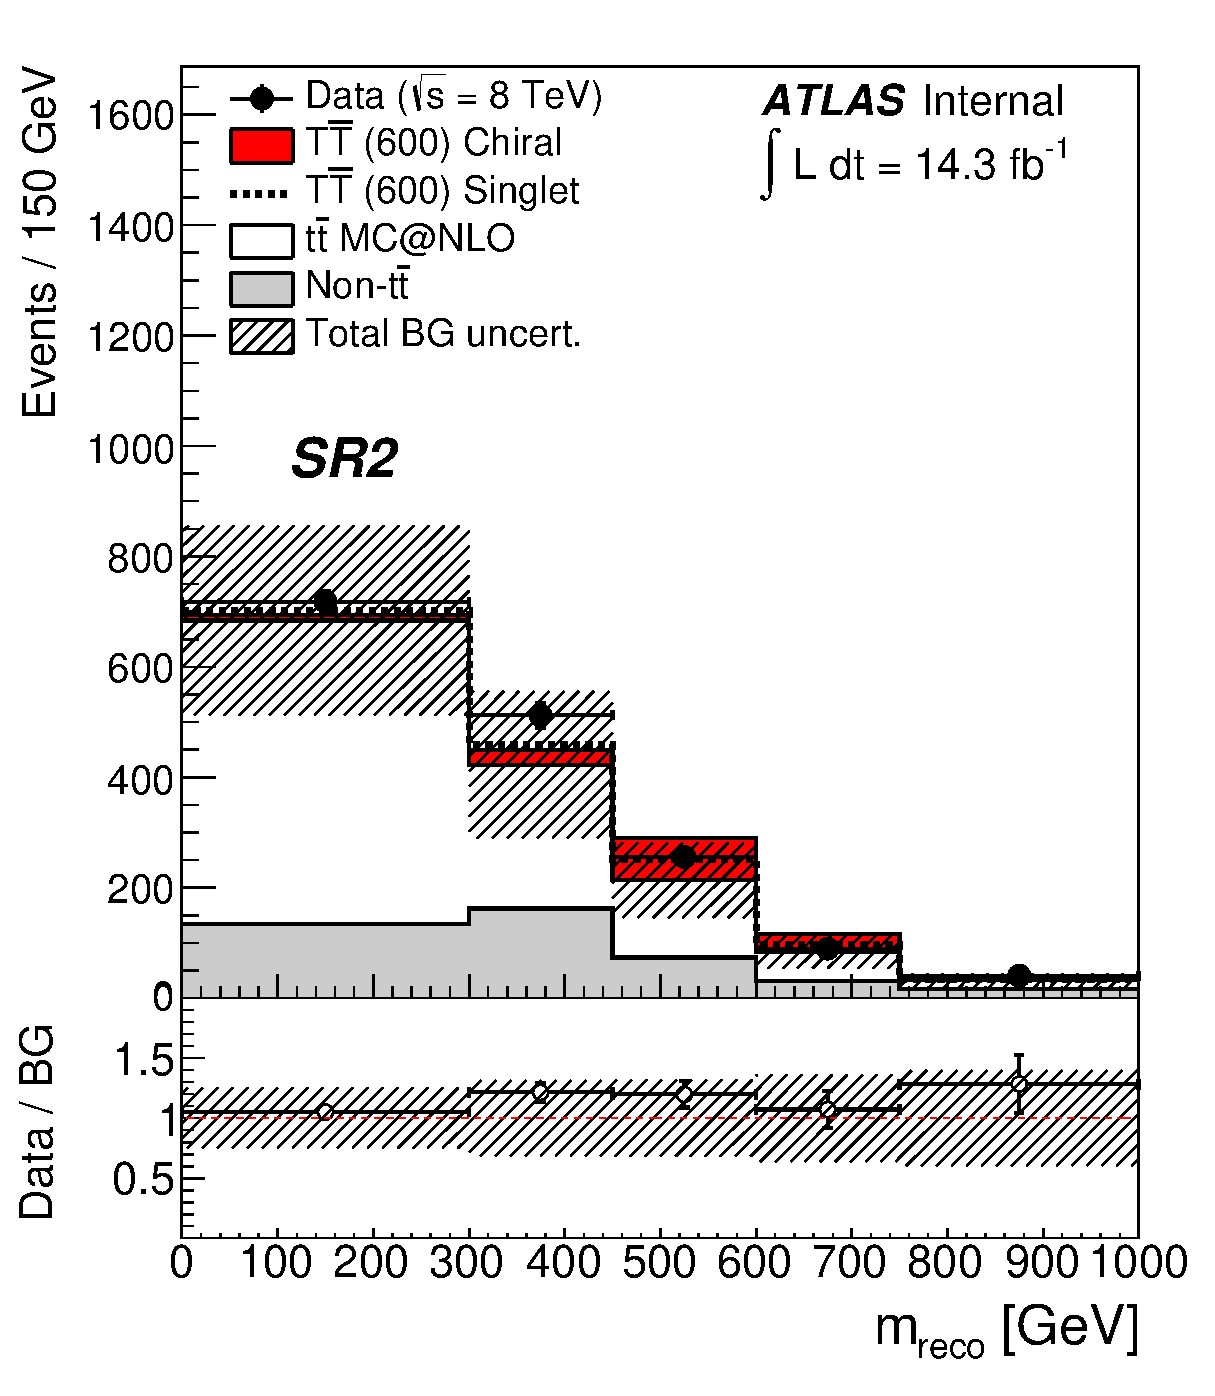
\includegraphics[width=0.37\textwidth]{wbx_analysis_14ifb/figures/THESIS_c6_cutflow/VLQAna_WbX_1W_MWb_4_ELEMUON_cutflow12_NOMINAL.eps}}
	\subfigure[]{\label{fig:mrecoSR3}
  	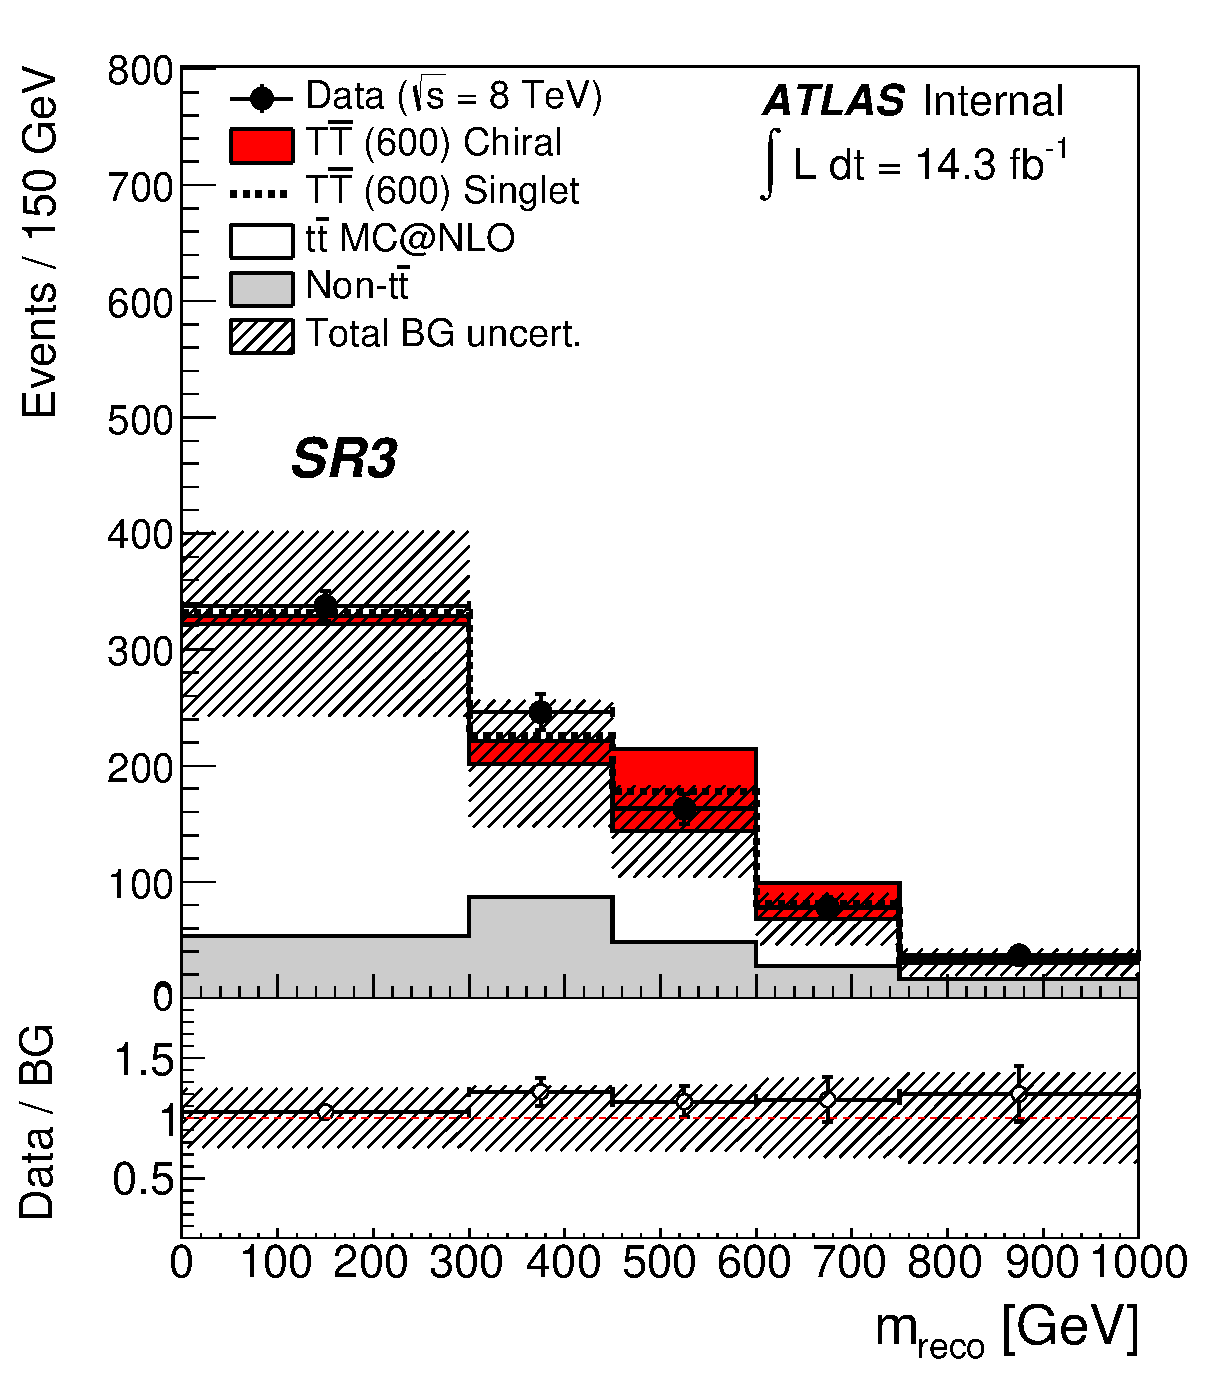
\includegraphics[width=0.37\textwidth]{wbx_analysis_14ifb/figures/THESIS_c6_cutflow/VLQAna_WbX_1W_MWb_4_ELEMUON_cutflow123_NOMINAL.eps}}
	\subfigure[]{\label{fig:mrecoSR4}
  	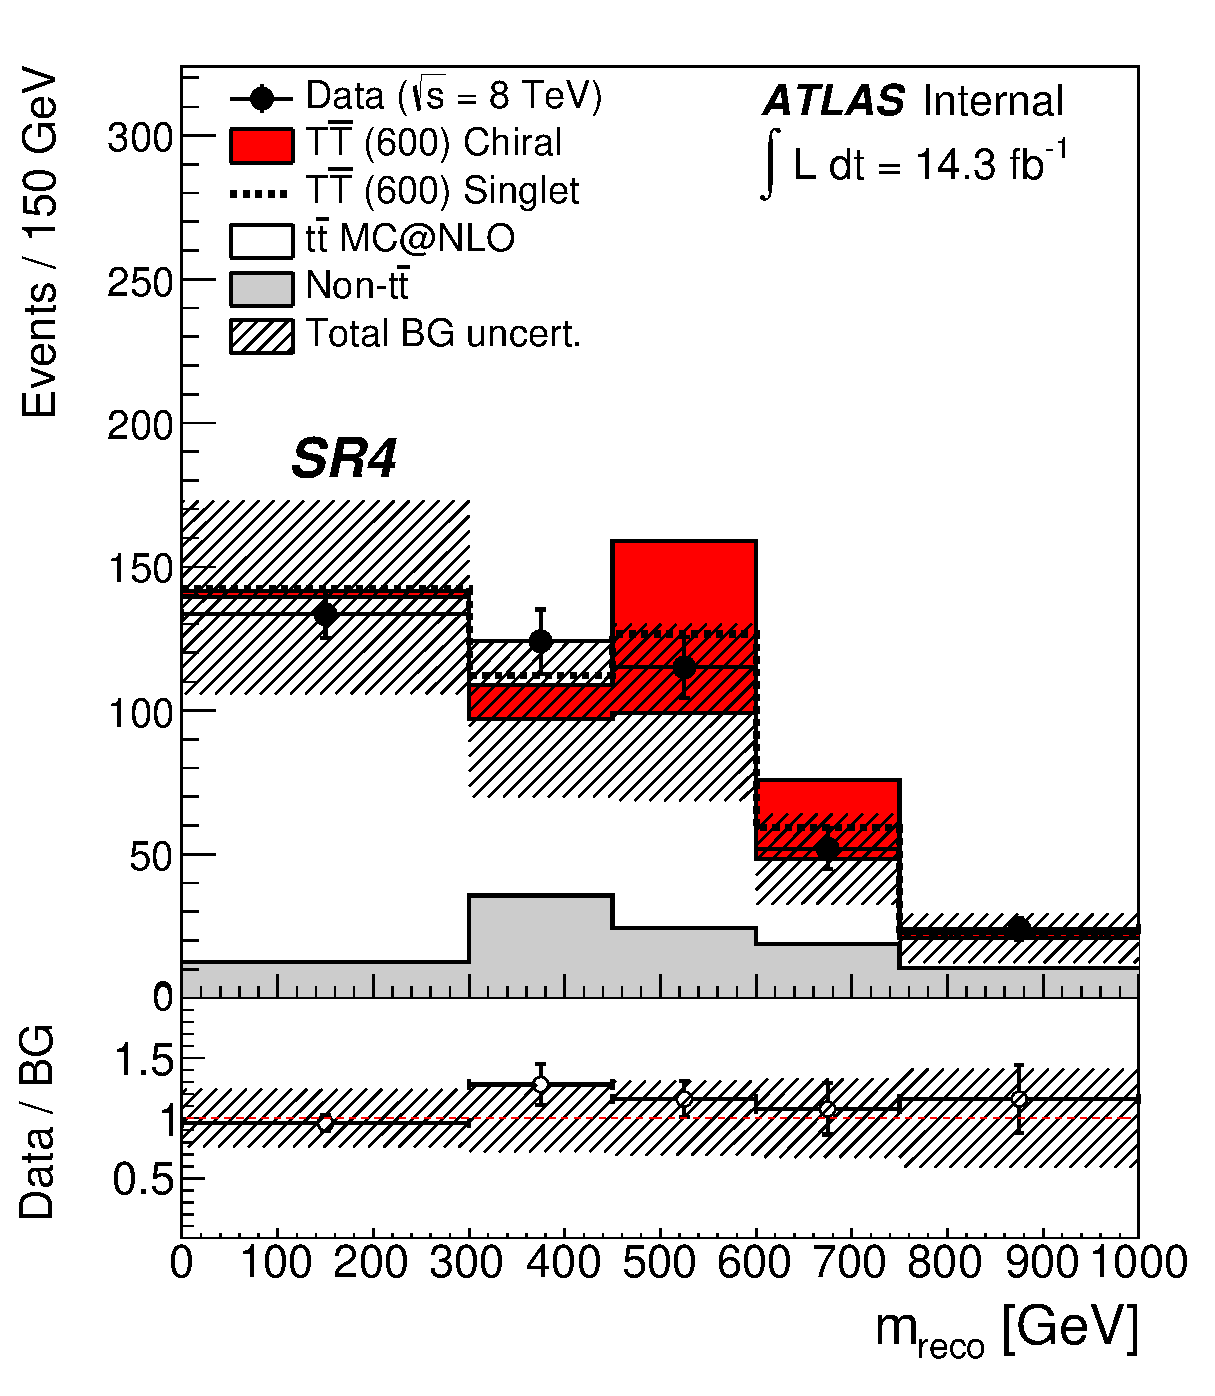
\includegraphics[width=0.37\textwidth]{wbx_analysis_14ifb/figures/THESIS_c6_cutflow/VLQAna_WbX_1W_MWb_4_ELEMUON_cutflow1234_NOMINAL.eps}}
	\subfigure[]{\label{fig:mrecoSR5}
  	\includegraphics[width=0.4\textwidth]{wbx_analysis_14ifb/figures/THESIS_c6_cutflow/VLQAna_WbX_1W_MWb_4_ELEMUON_cutflow12345_NOMINAL.eps}}
	\subfigure[]{\label{fig:mrecoSR6}
  	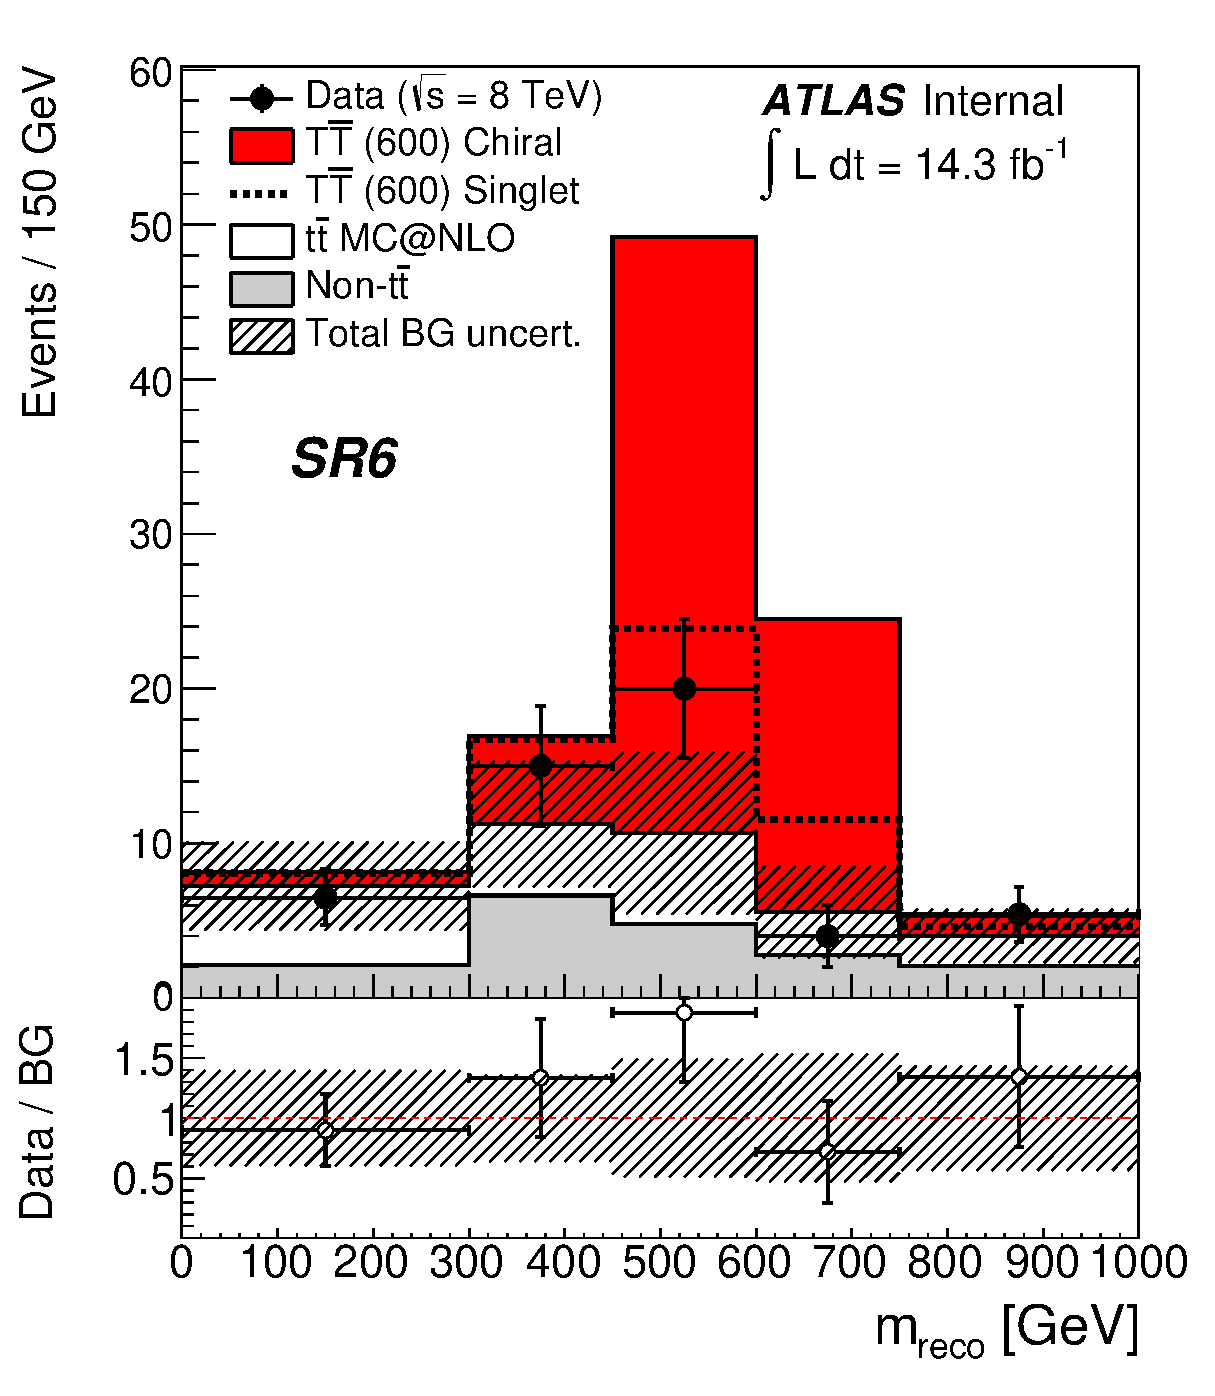
\includegraphics[width=0.4\textwidth]{wbx_analysis_14ifb/figures/THESIS_c6_cutflow/VLQAna_WbX_1W_MWb_4_ELEMUON_cutflow123456_NOMINAL.eps}}
	\subfigure[]{\label{fig:mrecoSR7}
  	\includegraphics[width=0.4\textwidth]{wbx_analysis_14ifb/figures/THESIS_c6_cutflow/VLQAna_WbX_1W_MWb_4_ELEMUON_cutflow1234567_NOMINAL.eps}}
	\caption[bla]{Distribution of the reconstructed mass \mreco\ in the combined
        electron and muon channel for the various signal regions: (a) SR1, (b) SR2,
        (c) SR3, (d) SR4, (e) SR5 also known as \loose\ selection, (f) SR6
        and (e) SR7 also known as \tight\ selection.
\input{wbx_analysis_14ifb/figures/confnoteplots/commoncaptionstack.tex}
\label{fig:mrecoSRs}}
\end{center}\end{figure}
\end{landscape}
